\documentclass{anstrans}
%%%%%%%%%%%%%%%%%%%%%%%%%%%%%%%%%%%%%%%%%%%%%%%%%%
\title{Use of Embree for ray tracing in the DAGMC toolkit}
\author{Patrick C. Shriwise, Andrew Davis, Paul P.H. Wilson}

\institute{University of Wisconsin-Madison, 1500 Engineering Dr, Madison, WI 53706, shriwise@wisc.edu}



%%%%% packages and defs
\usepackage{graphicx}
\usepackage{epsfig}

\begin{document}
%%%%%%%%%%%%%%%%%%%%%%%%%%%%%%%%%%%%%%%%%%%%%%%%%%
\section{Introduction}

The Direct Accelerated Geometry Monte Carlo (DAGMC) \cite{dagmc_2009} toolkit leverages the Mesh-Oriented datABase (MOAB) \cite{moab} to perform the geometric operations of Monte Carlo transport on CAD-based geometries. Ray-based operations such as point inclusion, next surface intersection, and surface normal determination are performed on nearly identical geometries with all the advantages of the design tools available in CAD software packages.

In the past, analysis using CAD-based geometry has saved man-hours in dealing with tedious and time-consuming geometric design methods, such as text-based geometries, at the cost of additional computational time. Efforts from developers at Intel are opening a pathway to a substantial decrease in this computational cost, leaving only the benefit of reduced human time and effort in the use of CAD-based geometries for analysis. 

This paper contains the preliminary results for an implementation of Intel's CPU-based ray tracing engine, Embree \cite{embree}, with DagMC for analysis with MCNP5 \cite{mcnp5} on several simple models, some specifically chosen for their complexity in the context of a ray tracing problem.

%%%%%%%%%%%%%%%%%%%%%%%%%%%%%%%%%%%%%%%%%%%%%%%%%%
\section{Spatial Partitioning Trees}

Spatial partitioning trees recursively subdivide the space bounded by a given set of data in order to quickly eliminate regions of the problem space irrelevant to the given query for the tree. These subdivisions come in many forms depending on the tree hierarchy being used. These are usually, but not always, binary trees.


\subsection{Bounding Volume Hierarchies}

Bounding volume hierarchies (BVHs) are a subset of a more general solution to the problem of a computational search for a point in 3D space known as spatial partitioning trees. In the case of BVHs, some closed volume is used to enclose these regions of 3D space, eventually leading to the enclosure of some number of primitive elements (in our case, triangles) to be queried for the desired geometric information. The most common BVHs use either oriented bounding boxes (OBBs) or axis-aligned bounding boxes (AABBs). AABBs will not conform as tightly to a generic set of data as OBBs. This lack of conformity can lead to increase inefficienty in the tree due to the overlapping of empty space for sibling bounding boxes. There is an additional cost, however, in using OBBs as bounding volumes. The transformation cost of the ray coordinates from the global proglem coordinates to the local OBB coordinates for the intersection check is considerable given the number of times this is done for even a single ray query. 

\subsection{Other Tree Hierarchies} 

Other bounding volumes and splitting conventions are also used in the are of spatial partitioning trees. For example, bounding spheres are sometimes used rather than boxes due to the simple and fast intersection check needed for ray queries. Hyperplane and hyperplane intervals are also used along each axis to subdivide data into a hierarchical structure. MOAB and Embree both use a BVH with bounding boxes so a detailed discussion of other spatial tree hierarchies will be neglected.

%%%%%%%%%%%%%%%%%%%%%%%%%%%%%%%%%%%%%%%%%%%%%%%%%%
\section{Intel's Embree}

Many existing ray tracing kernels use fine-grained, data dependent branching and irregular memory access which rules out other, more powerful optimiztaions like auto-vectorization. Embree's aim is to provide a CPU-based ray tracing kernel which combines the most efficient algorithms, data structures, and parallelization strategies for a given target architecture. Embree aims do do this for modern x86 architectures to access their full compute capability. In order to achieve this goal, Embree uses data structures and spatial splitting heuristics that allow for vectorization of spatial data structure traversals. \cite{embree} 

\subsection{Quad-branching Mixed BVH}

As mentioned above, most BVHs are binary trees, meaning each tree node has exactly 2 children with the exception of the leaf nodes. Embree uses a quad-branching tree (BVH4) in which each tree node has 4 children. While this increases the number of total nodes to traverse in the tree, Embree paralellizes the checking of these nodes, allowing for more exact exclusion of space in roughly the same time it would take for a check of 2 nodes in serial. 

Embree also employs what is referred to as a mixed BVH tree. Mixed BVH trees use a multitude of bounding volumes for construction. In particular, Embree uses the OBB and AABB mentioned in the bounding volume hierarchies section. In tree construction, AABBs are used to bound primitives only when deemed appropriate by deteriming if the local orientation of the triangles are closely algined with the global axes of the problem space. 

\subsection{Surface Area Heuristic}

There are many heuristics to be used when partitioning the the space contained by a bounding volume. In the past, most BVHs using bounding boxes have used median planar splitting. This planar splitting is usually done such that the ratio of surface area to volume is maximized (i.e. the volumes are kept more cubid) and the number of contained primitives is being split roughly in half to keep the expectation of performance like that of a standard binary tree search in the number of total primitives being contained. 

Recently there has been a new heuristic for partitioning bounding volumes and contained geometric primitives called the surface area heuristic (SAH) \cite{sah}. This heuristic is designed to minimize the cost $C$ of a split based on the number of primitives to be checked in each child, $P_{R}$ and $P_{L}$, at the cost, $C_{i}$, of a single primitive intersection check weighted by the size of the child boxes, $B_{r}$ and $B_{L}$, compared to the size of the parent box, $B$. There is an additional cost of the extra bounding volume intersection check implied by adding the cost of one traversal step down the tree, $C_{t}$.
Its formulation for a binary tree is as follows: 

\begin{equation} 
C = C_{t} + \frac{SA(B_{L})}{SA(B)} |P_{L}|C_{i} +  \frac{SA(B_{R})}{SA(B)} |P_{R}|C_{i}
\end{equation}

One can imagine this hueristic expanded to accomodate the quad-tree in Embree by adding two additional child terms idential to those of the left and right children represented in the binary tree case. This is what Embree does in the building of its mixed BVH4 hierarchy. 

\subsection{Floating Point Precision}

One aspect of Embree's speed is due to the use of float-precision rather than double-precision in its calculations. Currently, this is not typical of ray tracing systems used for Monte Carlo analysis, but for the sample cases tested for the purpose of this paper, the difference in precision does not manifest itself in the results. In the future, it is very possible that a double-precision version of Embree will exist \cite{gpu_mic_ray_tracing_rpi}, thus aleviating any concern of differences in results due to ray tracing calculations.

%%%%%%%%%%%%%%%%%%%%%%%%%%%%%%%%%%%%%%%%%%%%%%%%%%
\section{Implementation of Embree in DagMC}

Embree has been used in DagMC to replace the next surface, and point inclussion calculations for use in calculations using DAG-MCNP. This involves translating the mesh representation of the geometry in MOAB to an Embree instance. In Embree's native form, the ability to represent the underlying topological structure of a geometry-based mesh is limited. The ray tracing kernel is based on 'scenes' each scene being allowed to contain multiple 'geometries'. Even this relatively simple system allows for a one-to-one mapping of Embree geometries to MOAB surfaces and Embree scenes to MOAB volumes. Scenes cannot share mesh data, so surfaces are reproduced in this system for each volume they belong to. This duplication of surface mesh actually has its advantages as triangle normals in MOAB are adjusted on the fly based on which volume a current ray is in while the triangle normals can be pre-adjusted when creating the Embree geometries. This saves several computational steps when doing point inclusion calculations. Fortunately, Embree's mesh representation does not increase the memory footprint of DagMC greatly. Even if that were the case, once the Embree mesh representation has been properly established, the MOAB mesh could then be removed from memory.

In DagMC, particles on the surface of a volume are tracked by ignoring the near-surface intersection upon entering a new volume. This is done by ignoring triangles with normals opposing the current ray direction via a dot product result which is less than zero. In Embree, filter functions are used to emulate this process. Filter functions in Embree allow for a user-defined callback function for ray intersections. Embree will return its most recent valid intersection with all associated ray data (the hit triangle's unnormalized normal vector included) and allow a user to determine whether or not to accept the hit or instruct Embree to contiue the ray based on the outcome of the said filter function.

\subsection{Support for other applications}

Some spatial search operations needed by applications other than MCNP to be fully supported in DagMC are not natively supported by Embree, but due to Embree's allowance of direct access to their spatial tree structures, these functions can easily be implemented in a similar way to current ray intersection functions in Embree. In particular, this involves the implementation of a function for returning the closest intersetion to a given point in space.

\subsection{Ray Fire Timing: MOAB vs. Embree}

Several single-volume models have become the standard for testing ray fire timing of DagMC. These models include a single sphere, a sphere with notches cut into it, and a high-aspect ratio cylinder. Each of these models are meshed using increasingly smaller faceting tolerances to vary the number of triangles in the problem. The faceting tolerance is defined as the maximum distance between the faceted (meshed) curve or surface and the geometric curve or surface it resolves. 600,000 rays are fired from the origin of the geometry with an isotropic distribution in direction using the same random number seed to ensure amortization of the ray fire times.

\begin{figure}

  \begin{center}

    \epsfig{file=figs/sphere.ps,width=.3\columnwidth}
    \epsfig{file=figs/ds.ps,width=.3\columnwidth}
    \epsfig{file=figs/larcyl.ps,width=.3\columnwidth}
    \caption{The sphere, slotted sphere, and high aspect ration cylinder test models used for ray fire timings of MOAB and Embree. (left to right) }
    %\includegraphics{figs/sphere.ps}

  \end{center}

\end{figure}


Each model presents its own challenge with increating faceting tolerance. In the case of the sphere, the number of triangles in the generated mesh will always increase with decreasing faceting tolerance. This is not true of some geometries such as cubes or other rectuangular parallelpipeds. In the case of the notched sphere regions referred to as high-valance are generated as a result of faceting algorithms for planar surfaces meeting curved surfaces resulting in a single vertex connected to a high number of triangles. This is a difficult problem for BHVs to handle as the high triangle density usually results in large overlaps in the bounding volumes of the tree leading to inefficient tree traversals upon query. This problem tends to become exponentially worse as the faceting tolerance is decreased. The high aspect ratio cylinder will contain many small, skiny triangles running along the barrel of the cylinder. The particular shape of these triangles can cause problems in the calculations of tightly fiting OBBs used in MOAB to create spatial trees. This test model is used to determine the overall effectiveness of Embree's ability to use both OBBs and AABBs as well as the robustness of their OBBs algorithms for fitting to geometric objects with surface meshes of this nature.

\begin{figure}

  \begin{center}

    \epsfig{file=figs/hv.ps,width=.5\columnwidth}
    \caption{Example of the high-valence regions found in the slotted sphere at a high faceting tolerance (1e-04)}

  \end{center}

\end{figure}




\bibliographystyle{ans}
\bibliography{bibliography}


\end{document}
